\section{Bestimmung und Verifikation der Materialparameter}
\label{Kapitel:Parameter}
Um eine realistische Simulation zu ermöglichen, ist es notwendig die verwendeten Mo\-delle möglichst genau an Rheometer-Messdaten der realen Mörtel anzupassen. Dazu können die materialabhängigen Parameter in den Modellen variiert werden.
Für einige der Mörtel wurden die Parameter, die im verwendeten Herschel-Bulkley Modell~\eqref{eq:modHB} vorkommen, schon in früheren Arbeiten bestimmt.
Für die Bestimmung aktueller und zukünftiger Mörtel  wurde entschieden, Programme für Simulation und Optimierung zu verwenden, die unabhängig von Drittanbietern in Form von Lizenzen und Support sind.
%Einerseits wurden aber in der Zwischenzeit neue Mörtel entwickelt und andererseits ist es wünschenswert, ein Tool zur automatischen Bestimmung dieser Parameter zu haben, das unabhängig von Drittanbietern in Form von Lizenzen und Support ist.
Dies wurde mithilfe einer Kombination aus \openfoam{} und der Programmiersprache Python umgesetzt.
%
\subsection{Rheometer}
\label{Kapitel:Rheometer}
Rheometer sind Messgeräte, mit denen man die Fliesskurve von nicht-Newtonschen Fluiden experimentell bestimmen kann.
Dabei wird das Fluid in eine stationäre, laminare Schichtenströmung versetzt. Dadurch ist es möglich, anhand einer
Messgrösse die Viskosität abhängig von der Scherrate zu bestimmen.
Die Messungen wurden von einem Hilti-internen Rheo\-logen durchgeführt. Verwendet wurden zwei Messgeräte, ein Platte-Platte Rheometer und ein Kapillarrheometer.
%
\subsubsection{Platte-Platte Rheometer}
\label{Kapitel:Parameter:PlattePlatteRheo}
Das Platte-Platte Rheometer besteht aus zwei zylindrischen Platten, die so montiert sind, dass zwischen ihnen ein schmaler, ebenfalls zylinderförmiger Spalt entsteht (Abbildung~\ref{fig:platteRheoSchema:subA}).
\begin{figure}[tb]
    \centering
    \subfloat[Platte-Platte Rheometer ohne Ring]{
    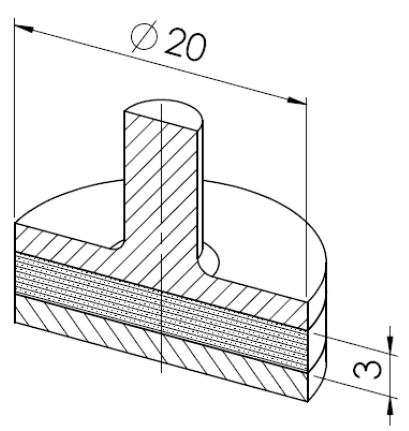
\includegraphics[width=0.45\textwidth]{figures/PlatteOhneRing.PNG}
    \label{fig:platteRheoSchema:subA}
    }
    \subfloat[Platte-Platte Rheometer mit Ring]{
    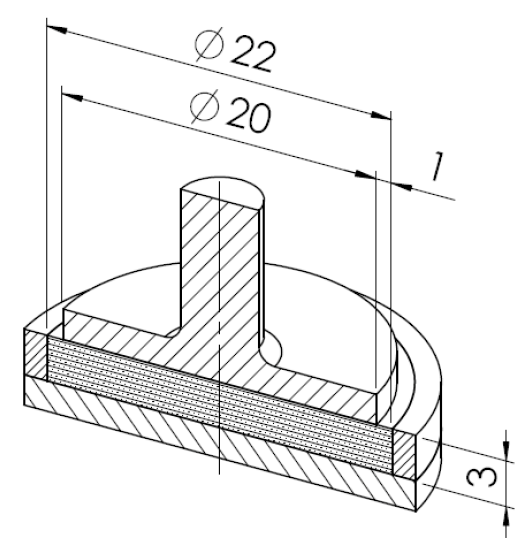
\includegraphics[width=0.45\textwidth]{figures/PlatteMitRing.png}
    \label{fig:platteRheoSchema:subB}
    }
    \caption{Eine schematische Darstellung des Platte-Platte Rheometers. In \subref{fig:platteRheoSchema:subA} ist die Version ohne den Ring zu sehen, in \subref{fig:platteRheoSchema:subB} umschliesst ein Ring den Scherspalt, um ein Herausfliessen des Mörtels zu verhindern. Die Distanzen sind in Millimeter angegeben.\\
    Bildquelle: \cite{Marco}.}
    \label{fig:kapRheo}
\end{figure}
Die Flüssigkeit wird in diesem Scherspalt platziert, der in radialer Richtung von einem Ring abgeschlossen werden kann. Beim Messvorgang wird die eine Platte fixiert, die andere mit einer vorgegebenen Geschwindigkeit $\omega$ gedreht.
Dabei wird das Drehmoment gemessen, das für die Drehgeschwindigkeit aufgewendet werden muss.

Die zur Auswertung der Viskosität aus dem Drehmoment verwendete Formel lautet
\begin{equation}
    \label{eq:platterheovisko}
    \eta\left( \gammap \right) = \frac{2M}{\pi R^3 \gammap}\left( \frac{3+n}{4} \right)\quad\text{mit}\quad n=\frac{d\ln M}{d\ln\gammap}~.
\end{equation}
Dabei ist \nom[rv:M]{$M$}{Drehmoment} das benötigte Drehmoment und \nom[rv:R]{$R$}{Plattenradius des Platte-Platte Rheometers} der Radius der verwendeten Platten
%Für eine Herleitung dieser Formel wird auf \cite{introtorheo} verwiesen.
\cite{introtorheo}.

Das Platte-Platte Rheometer eignet sich auch dazu, zeitabhängige Effekte wie die Relaxationszeit eines viskoelastischen Fluids zu messen.
Dazu wird die obere Platte nicht mit einer konstanten Geschwindigkeit bewegt, sondern mit einer oszillierenden Drehung auf die eine oder die andere Seite bewegt.
Bei diesem Vorgang, der Oszillationsmessung genannt wird, kann anhand der resultierenden, nicht stationären Strömung über die Messung des Widerstandes eine Abschätzung der Schwingungsmodi der Flüssigkeit getroffen werden.

Die sinusförmige Deformation \nom[gv:gamma]{$\gamma$}{Scherung} des Fluides verursacht dabei einen ebenfalls sinusförmigen Widerstand, der durch eine Schubspannung \nom[gv:tau]{$\tau$}{Schubspannung} im Fluid zustandekommt.
Bei einem ideal viskosen Fluid ist dieser Widerstand zur Deformation um \ang{90} phasenverschoben. Das liegt daran, dass der Widerstand proportional zur Schergeschwindigkeit $\gammap$ der Flüssigkeit ist.
Bei einem ideal elastischen Material ist der Widerstand in Phase mit der Deformation, da er direkt proportional zur Verzerrung $\gamma$ des Materials ist.

Ein viskoelastisches Fluid besitzt die Eigenschaften beider Materialien und hat deshalb einen Antwort-Widerstand, der um einen Winkel zwischen \ang{0} und \ang{90} phasenverschoben ist. Der Betrag der Verschiebung hängt dabei vom Verhältnis der viskosen und der elastischen Anteile des Fluids ab. Dieser Zusammenhang ist in Abbildung~\ref{fig:schwingungsmodi} dargestellt.

Diese Beziehungen können als Zusammenhang zwischen Schubspannung $\tau$ und Zeit $t$ ausgedrückt werden:
\begin{align}
    \label{eq:schwingungsmodi}
    \tau\left( t \right)&=G'\cdot\hat{\gamma}\cdot \sin\left( \omega\cdot t \right) && \text{elastisch}\\
    \tau\left( t \right)&=\eta\cdot\omega\cdot\hat{\gamma}\cdot \cos\left( \omega\cdot t \right)&& \text{viskos}\\
    \tau\left( t \right)&=G'\cdot\hat{\gamma}\cdot \sin\left( \omega\cdot t \right)+G''\cdot\hat{\gamma}\cdot \cos\left( \omega\cdot t \right)&& \text{viskoelastisch}
\end{align}
Dabei ist \nom[gv:omega]{$\omega$}{Kreisfrequenz} die Kreisfrequenz und \nom[rv:gammah]{$\hat\gamma$}{Scherungsamplitude beim Platte-Platte Rheometer} die Amplitude der am Rheometer angelegten Schwingung. $\eta$ ist die Viskosität des Fluids und \nom[rv:Gs]{$G'$}{Elastizitätsmodul} das Elasti"-zi"-tätsmodul des elastischen Materials. Der Term $\eta\cdot\omega$ wird auch als Verlustmodul \nom[rv:Gss]{$G''$}{Verlustmodul} bezeichnet. Dabei bestimmt das Elastizitäts- und das Verlustmodul, wieviel Energie als elastische Energie gespeichert wird und wieviel davon dissipiert wird.

Anhand der aus den Messungen resultierenden Grössen $G'$ und $G''$ können die viskoelastischen Eigenschaften wie z.B. die Relaxationszeit eines Fluids bestimmt werden.

\begin{figure}[h]
    \centering
    \subfloat[Auslenkung $\gamma$ und Schergeschwindigkeit $\gammap$]{
    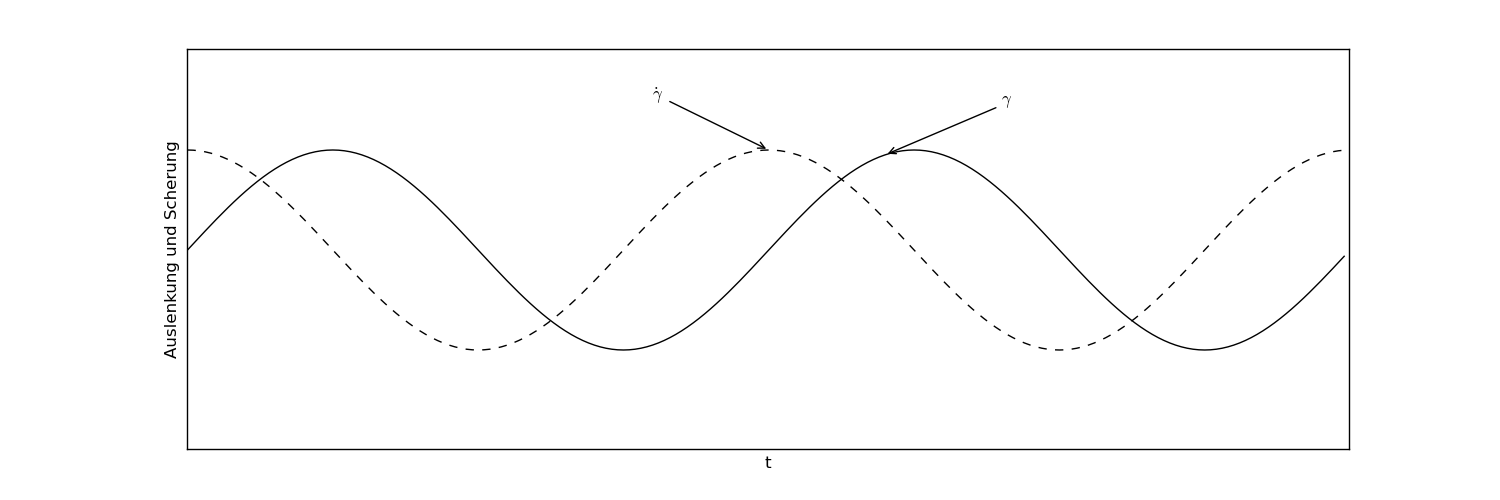
\includegraphics[width=\textwidth]{figures/SchwingungsmodiA.png}
    \label{fig:schwingungsmodi:subA}
    }\\
    \subfloat[Reaktion des Materials]{
    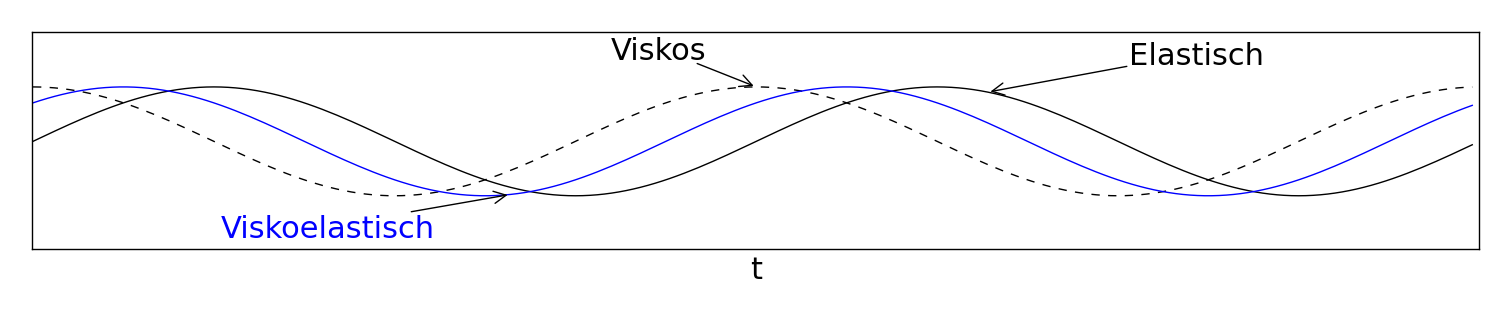
\includegraphics[width=\textwidth]{figures/SchwingungsmodiB.png}
    \label{fig:schwingungsmodi:subB}
    }
    \caption{Oszillationsversuch mit dem Platte-Platte Rheometer.\\
    In \subref{fig:schwingungsmodi:subA} ist die sinusförmige Auslenkung $\gamma$ als durchgezogene Linie, die resultierende Schergeschwindigkeit $\gammap$ als gestrichelte Linie gezeichnet.\\
    In \subref{fig:schwingungsmodi:subB} ist die Reaktion des Materials auf die Auslenkung dargestellt. Ein elastisches Material hat einen Widerstand in Phase mit der Auslenkung, eine viskose Flüssigkeit ist um \ang{90} phasenverschoben. Ein viskoelastisches Material liegt zwischen diesen beiden Kurven.
    }
    \label{fig:schwingungsmodi}
\end{figure}
%
\subsubsection{Kapillarrheometer}
Das Kapillarrheometer kann wie das Platte-Platte Rheometer zur Bestimmung der scherratenabhängigen Viskosität verwendet werden. Das Fluid wird dabei aber nicht gedreht, sondern durch eine zylinderförmige Kapillare gepresst. Als Messgrösse dient dann der Druckunterschied.
Um dabei den durch das Mitmessen des Einlaufdruckverlustes (Bagley-Druck) gemachten systematischen Fehler zu korrigieren, wird meistens parallel zum eigentlichen Kapillarrheometer auch noch der Druckverlust in einer Nullblende gemessen, wie in Abbildung~\ref{fig:kapRheo} dargestellt.
\begin{figure}[tbh]
    \centering
    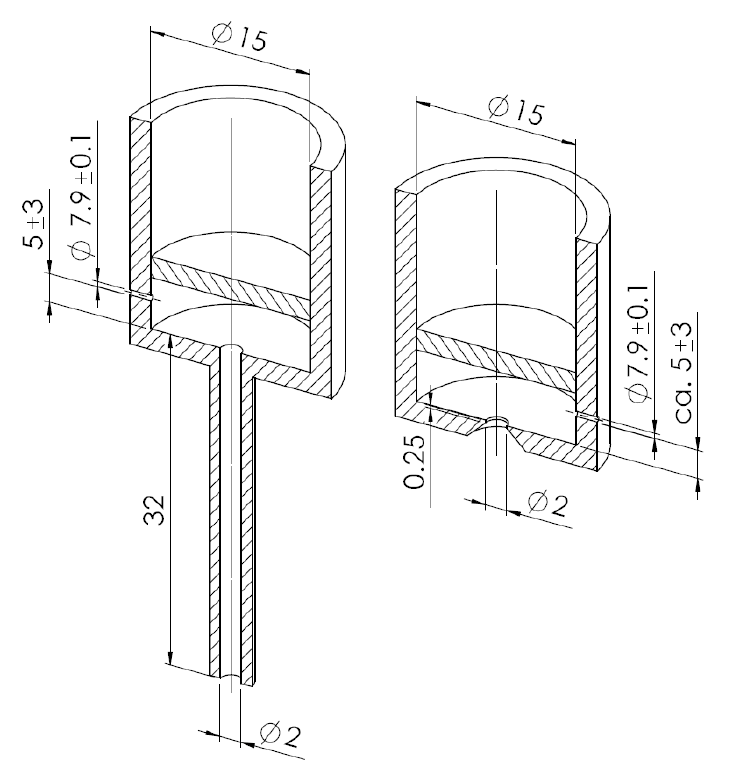
\includegraphics[height=10cm]{figures/KapRheo.png}
    \caption{Eine schematische Darstellung des Kapillarrheometers. Links ist der Einlaufkolben mit anschliessender Kapillare zu sehen, rechts der Einlaufkolben ohne Kapillare zur Messung des Bagley-Druckes.
    Bildquelle: \cite{Marco}.}
    \label{fig:kapRheo}
\end{figure}

Die Beziehung der Messgrösse \nom[rv:pmess]{$\Delta p_{\mbox{\tiny Mess}}$}{Gemessener Druckverlust beim Kapillarrheometer} zu der Schubspannung $\tau$ ist dabei wie folgt:
\nomenclature[rv:pbagley]{$\Delta p_{\mbox{\tiny Bagley}}$}{Einlaufdruckverlust beim Kapillarrheometer}
\begin{equation}
    \label{eq:KapRheoTau}
    \tau\left( R_{\mbox{\tiny Kap}} \right) = \frac{R_{\mbox{\tiny Kap}} \Delta p}{2L_\text{\tiny Kap}},
\end{equation}
wobei $\Delta p = \Delta p_{\mbox{\tiny Mess}} -\Delta p_{\mbox{\tiny Bagley}}$ der korrigierte Druckunterschied ist und \nom[rv:Lkap]{$L_\text{\tiny Kap}$}{Länge des Kapillarrheometers} und \nom[rv:Rkap]{$R_\text{\tiny Kap}$}{Kapillarradius des Kapillarrheometers} die Länge, respektive der Radius der Kapillare sind.

Für die Berechnung der in der Kapillare auftretenden Scherrate kann die Beziehung
\begin{equation}
    \label{eq:KapRheoScherrate}
    \gammap = \frac{4 \dot{V}}{\pi R^3}\left( \frac{3+n}{4} \right)\quad\mbox{mit}\quad n=\frac{d \ln \dot{V}}{d\ln\tau}
\end{equation}
verwendet werden. 

Mit Hilfe von \eqref{eq:KapRheoTau} und \eqref{eq:KapRheoScherrate} lässt sich die Fliesskurve 
\begin{equation}
    \eta(\gammap) = \frac{\tau}{\gammap}
\end{equation}
abhängig vom gemessenen Druckunterschied und vorgegebenen Volumenstrom \nom[gv:Vdot]{$\dot{V}$}{Volumenstrom} bestimmen.
%
%
\subsection{Korrektursimulation}
\label{Kapitel:Korrektursimulation}
Das in Kapitel \ref{Kapitel:Parameter:PlattePlatteRheo} beschriebene Rheometer misst das für eine vorgegebene Geschwindigkeit benötigte Drehmoment. Daraus kann nach \eqref{eq:platterheovisko} die Vis\-ko\-si\-tät des Fluides berechnet werden.
Um zu verhindern, dass der Mörtel während der Messung in radialer Richtung aus dem Gerät fliesst, wurde um den Scherspalt ein Ring montiert (Abbildung~\ref{fig:platteRheoSchema:subB}). Dadurch wird zwar ein Herausfliessen verhindert, gleichzeitig wird aber die Messung verfälscht. Der Ring ist eine zusätzliche Wand an der das Fluid entlangströmen muss. Die Wandhaftung hat ein erhöhtes Drehmoment zur Folge, was dazu führt, dass in der Berechnung der Viskosität ein systematischer Fehler gemacht wird.
Um trotzdem eine zuverlässige Bestimmung der Viskosität zu ermöglichen, ist es notwendig, diesen Ring zu berücksichtigen. 
Dazu wird in einer Simulation das reale System, also mit Ring, abgebildet und berechnet. 
Die Viskosität in der Simulation hängt vom Herschel-Bulkley Modell~\eqref{eq:modHB} ab, das durch Materialparameter bestimmt ist. Diese werden nun so lange variiert, bis Messung und Simulation dasselbe Drehmoment ergeben.
Dieser Vorgang ist in Abbildung~\ref{fig:korrekturSim} verdeutlicht.
%
\begin{figure}
    \centering
    \tikzstyle{block} = [rectangle, draw, fill=blue!10, 
    text width=5em, text centered, rounded corners, minimum height=4em]
    \tikzstyle{line} = [draw, -latex']
    \tikzstyle{cloud} = [draw, circle, node distance=3cm,
    minimum height=2em]
    \begin{tikzpicture}[node distance = 2cm, auto]
        \node[block] (init) {Messung};
        \node[block, below of=init] (cfd) {Simulation};
        \path (init) -- (cfd) node[midway] (m) {};
        \node[cloud, right of=m] (d) {d};
        \node[cloud, left of=m] (omeg) {$\omega$};
        \node[block, text width=10em, node distance = 4cm, right of=d] (opt) {Optimierung};
        %
        \path[line] (init) -| (d) node[above,pos=0.4] {M Messung};
        \path[line] (cfd) -| (d) node[below,pos=0.4] {M Simulation};
        \path[line] (omeg) |- (init) ;
        \path[line] (omeg) |- (cfd) ;
        \path[line] (d) -- (opt) ;
        \path[line] (opt) |- ++(-4cm,-2.5cm) node[below] {Neue Parameter} -| (cfd) ;
    \end{tikzpicture}
    \caption{Schematischer Ablauf für die Korrektur des systematischen Fehlers bei der Platte-Platte Rheometer-Messung}
    \label{fig:korrekturSim}
\end{figure}

Simuliert wurde das Platte-Platte Rheometer, mit einer Haftbedingung an der unteren Platte und am Ring, einer konstanten Dreh"-ge"-schwin"-dig"-keit $\omega$ und einem offenen Spalt zwischen oberer Platte und dem Ring (Abbildung~\ref{fig:plattenRheoRand:subB}).
Beim Platte-Platte Rheometer handelt es sich um eine rotationssymmetrische Geometrie. Um Rechenzeit zu sparen wurde deshalb nur ein Kreissegment der Geometrie, ergänzt um periodische Rand"-bedingungen, simuliert. In Abbildung~\ref{fig:plattePlatteRheoSim} ist ein Farbplot der resultierenden Ge"-schwin"-dig"-keits"-ver"-tei"-lung mit und ohne Ring gezeigt.
%
\begin{figure}[bt]
    \centering
    %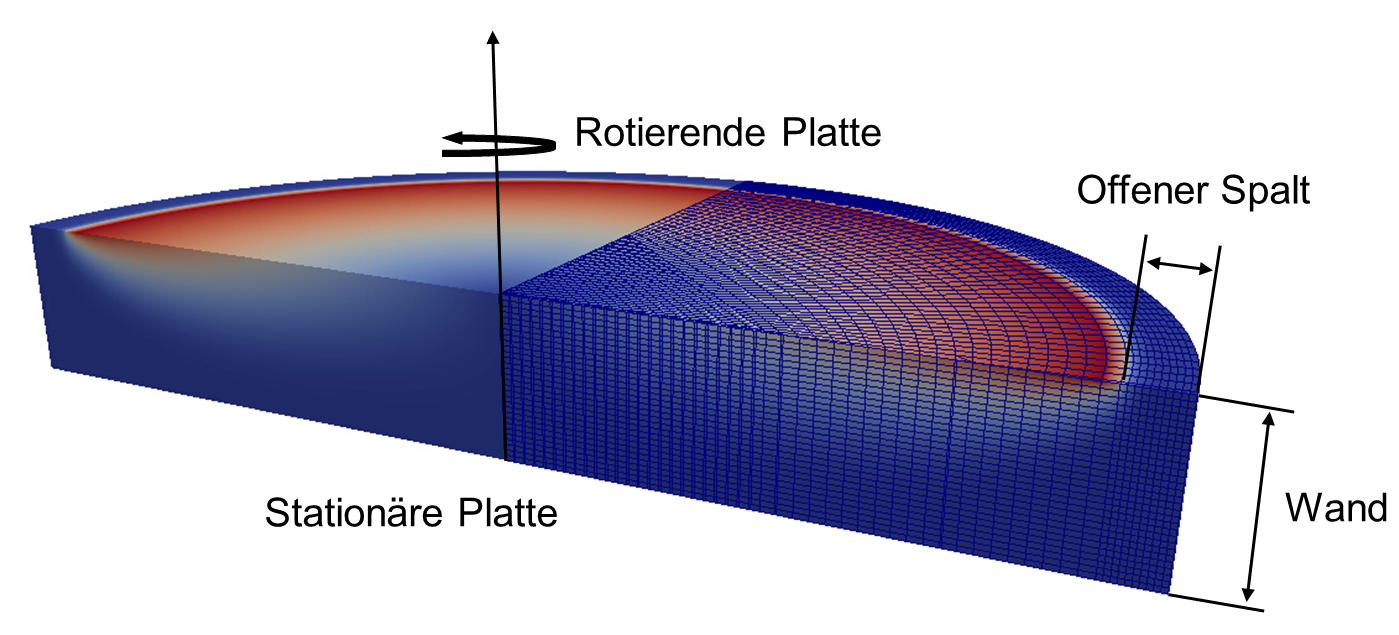
\includegraphics[width=\textwidth]{figures/plattenRheoFullCircAnnot.png}
    \subfloat[Ohne Ring]{
    \begin{tikzpicture}[scale=0.7]
        \draw[fill=lightgray] (0,0) -- ++ (5,0) -- ++ (0,2) -- ++ (-5,0) -- ++ (0,-2);
        \draw[ultra thick,<->] (1,0) -- (0,0) -- (0,1);
        \node[left] at (0,1) {z};
        \node[below] at (1,0) {r};
        \node[below] at (3,0) {$\u=0$};
        \node[below] at (5,0) {R};
        \node[right] at (5,1) {$\frac{\partial\u}{\partial r}=0$};
        \node[above] at (3,2) {$\u=r\cdot\omega$};
    \end{tikzpicture}
    \label{fig:plattenRheoRand:subA}
    }
    \subfloat[Mit Ring]{
    \begin{tikzpicture}[scale=0.7]
        \path[fill=lightgray] (0,0) -- ++ (5,0) -- ++ (0,2) -- ++ (-5,0) -- ++ (0,-2);
        \draw[fill=lightgray] (5,0) -- ++ (1,0) -- ++ (0,2) -- ++ (-1,0) ;
        \draw (0,0) -- ++ (5,0) -- ++ (0,2) -- ++ (-5,0) -- ++ (0,-2);
        %\draw (6,0) -- (6,2);
        \draw[ultra thick,<->] (1,0) -- (0,0) -- (0,1);
        \node[left] at (0,1) {z};
        \node[below] at (1,0) {r};
        \node[below] at (3,0) {$\u=0$};
        \node[below] at (5,0) {R};
        \node[below right] at (6,0) {R+S};
        \node[right] at (6,1) {$\u=0$};
        \node[above] at (3,2) {$\u=r\cdot\omega$};
        \node[above] at (5.5,2) {$\frac{\partial\u}{\partial r}=0$};
    \end{tikzpicture}
    \label{fig:plattenRheoRand:subB}
    }
    \caption{Randbedingungen für die Simulation des Platte-Platte Rheometers. An der stationären Platte und der Wand gilt $\u=0$, die rotierende Platte besitzt die vorgegebene Geschwindigkeit $\u=r\cdot\omega$ und an den freien Oberflächen wird Umgebungsdruck vorgegeben.}
    \label{fig:plattenRheoRand}
\end{figure}
%
\begin{figure}
\centering
\subfloat[Ohne Ring]{
\begin{tikzpicture}[inner sep=0pt]
    \node at (0,0) {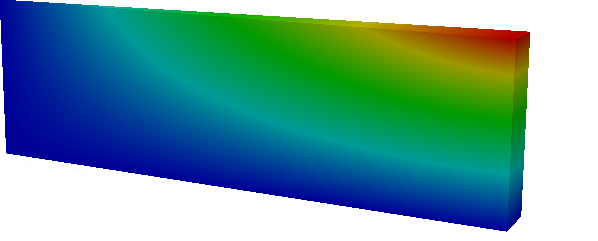
\includegraphics[width=.45\textwidth]{figures/platteRheoSimOhneRing.png}};
    \draw[thick] (-3.06,1.22) --++ (0,0.2) node[pos=0.5](olA){};
    \draw[thick] (2.37,0.88) --++  (0,0.2) node[pos=0.5](orA){};
    \draw[thick] (2.37,0.88) --++  (0.2,0) node[pos=0.5](roA){};
    \draw[thick] (2.28,-0.99) --++  (0.2,0) node[pos=0.5](ruA){};
    \draw[thick,<->] (olA) -- (orA) node[pos=0.5,inner sep=2pt,above]{R};
    \draw[thick,<->] (roA) -- (ruA) node[pos=0.5,inner sep=2pt,right]{H};
\end{tikzpicture}
\label{fig:platteRheoSim:subA}
}
\subfloat[Mit Ring]{
\begin{tikzpicture}[inner sep=0pt]
    \node at (0,0) {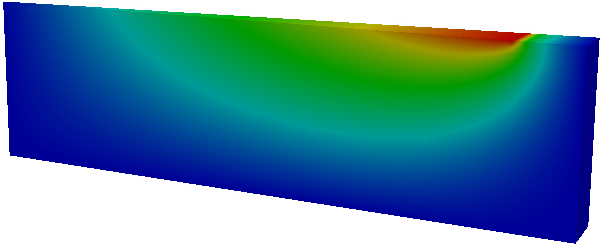
\includegraphics[width=.45\textwidth]{figures/platteRheoSimMitRing.png}};
    \draw[thick] (-3.04,1.22) --++ (0,0.2) node[pos=0.5](olB){};
    \draw[thick] (3.05,0.875)--++  (0,0.2) node[pos=0.5](orB){};
    \draw[thick] (3.05,0.875)--++  (0.2,0) node[pos=0.5](roB){};
    \draw[thick] (2.95,-1.03)--++  (0.2,0) node[pos=0.5](ruB){};
    \path (olB) -- (orB) node[pos=0.889](omB){};
    \draw[thick] (omB) -- ++ (0,0.1) -- ++ (0,-0.2);
    \draw[thick,<->] (olB) -- (omB) node[pos=0.5,inner sep=4pt,above]{R};
    \draw[thick,<->] (omB) -- (orB) node[pos=0.5,inner sep=4pt,above]{S};
    \draw[thick,<->] (roB) -- (ruB) node[pos=0.5,inner sep=2pt,right]{H};
\end{tikzpicture}
%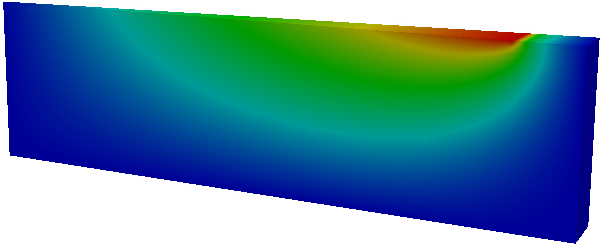
\includegraphics[width=.45\textwidth]{figures/platteRheoSimMitRing.png}
\label{fig:platteRheoSim:subB}
}
\caption{Simulierter Teil des Platte-Platte Rheometers, in \subref{fig:platteRheoSim:subA} ohne Ring, in \subref{fig:platteRheoSim:subB} mit Ring.
Eingefärbt ist das Bild nach der resultierenden Geschwindigkeitsverteilung im Rheometer.}
\label{fig:plattePlatteRheoSim}
\end{figure}
%
\subsubsection{Optimierung}
Die in Abbildung~\ref{fig:korrekturSim} gezeigte Optimierung der Parameter ist ein nicht\-li\-neares Ausgleichsproblem. Dabei soll die Gleichung \eqref{eq:modHB} möglichst gut an Mess- und Simulationsdaten angepasst werden, indem die Parameter $\tau_0$, $K$ und $n$ variiert werden.
Für die Lösung dieses Ausgleichproblems wurde die Programmiersprache Python verwendet. Die Tatsache, dass Python, ebenso wie \openfoam{}, frei verfügbar ist und dass es eine grosse Anzahl schon implementierter numerische Algorithmen gibt, macht Python zur idealen Wahl.

Die Optimierung wurde als Python Modul \codeemph{MaT\_Optimizer} implementiert. Dabei wurde auf die Bibliotheken \codeemph{Numpy} und \codeemph{Scipy} \cite{scipy} zurückgegriffen, um eine Reihe mathematischer Standardfunktionen zur Verfügung zu haben.
Das Ausgleichsproblem wird dabei mittels der Funktion \codeemph{leastsq} aus dem Modul \codeemph{optimize} von \codeemph{Scipy} gelöst.
Diese Funktion ist eine Implementierung des Levenberg-Marquardt Algorithmus, der das Problem auf eine iterative Weise löst.
Da während dieser Iterationen laufend neue Simulationen durchgeführt werden müssen, wird eine enge Kopplung von Python und \openfoam{} benötigt.
%da die Auswertung der Funktion, an die gefittet werden soll, eine Reihe von Simulationen ist.
Diese Kopplung wurde dabei mit Hilfe von \codeemph{PyFoam} \cite{pyfoam} realisiert. \codeemph{PyFoam} ist eine Python Bibliothek, die es ermöglicht, die von \openfoam{} als Ein- und Ausgabe benutzten Textdateien auf einfache Art und Weise zu erzeugen, zu ändern und auszulesen.
Um den Prozess der Parameter Optimierung zu beschleunigen, wurde ausserdem die Bibliothek \codeemph{Parallel Python} \cite{parallelpython} verwendet. Da eine Funktions"-auswertung mehrere Simulationen beinhaltet, wird dazu viel Zeit benötigt. Diese Simulationen sind aber unabhängig voneinander und können deshalb sehr einfach parallelisiert werden. Mit \codeemph{Parallel Python} können beliebig viele Prozessoren für den Parameterfit verwendet werden.

%In Kapitel~\ref{Kapitel:Korrektursimulation} wird beschrieben, wie die Korrektursimulation für das Platte-Platte Rheometer angewendet wird.
Die gemessenen Daten des Kapillarrheometers werden bereits bei der Messung durch die Verwendung des Bagley-Druckes korrigiert.
Falls diese in die Optimierung mit einbezogen werden sollen, muss also keine Korrektur\-simulation durch"-geführt werden; die Daten können direkt für die Optimierung verwendet werden. 
Dies wird im Python Code berücksichtigt, indem der Unterschied zwischen gemessenen und aus den Modell-Parametern berechneten Druckunterschieden direkt an die Fehlerfunktion angehängt wird.

Die genaue Dokumentation des \codeemph{MaT\_Optimizer} Moduls findet sich in Anhang~\ref{Appendix:Python}.
%
\subsubsection{Gitterkonvergenz}
Da die Rechenzeit einer einzelnen Simulation durch die hohe Anzahl an Simulationen sehr stark ins Gewicht fällt, wurde versucht ein möglichst grobes Netz zu verwenden. Natürlich wird dadurch der Diskretisierungsfehler immer grösser, weshalb ein Kompromiss zwischen benötigter Simulationszeit und gemachtem Fehler gefunden werden musste.
Dazu wurde das resultierende Drehmoment bei der Verwendung verschiedener Netze verglichen.  
Das verwendete Netz, dargestellt in Abbildung~\ref{fig:PlatteRheoGitter}, ist ein he\-xa\-edri\-sches Gitter mit einer Zelle in tangentialer Richtung und einer Diskreti"-sierungslänge von $2^{-h} \cdot 0.2\mbox{mm}$, wobei $h\in\left\{ 0,1,2,3 \right\}$. Erstellt wurde das Netz mit dem in \openfoam{} vorhandenen Netzer \codeemph{blockMesh}.
%
\begin{figure}[tb]
    \centering
    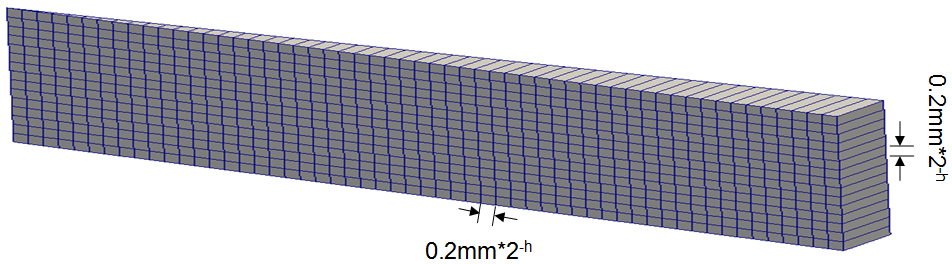
\includegraphics[width=\textwidth]{figures/PlatteRheoGitterAnnot.png}
    \caption{Das verwendete Gitter für die Simulation des Platte-Platte Rheometers. Der Parameter $h$ wurde zwischen 0 und 3 variiert.}
    \label{fig:PlatteRheoGitter}
\end{figure}
%
Die resultierenden Werte für das Drehmoment sind in Tabelle \ref{fig:ResultingTorque} aufgeführt. Aufgrund der hohen Rechenzeit für feinere Auflösungen wurde entschieden, die Simulationen mit dem Netz $h=1$ durchzuführen.
%
\begin{table}[tbh]
    \centering
    \begin{tabular}{l c c c c}
        %\toprule
        \textbf{h} & 0 & 1 & 2 & 3\\
        \midrule
        \textbf{M} & $1.4178\cdot10^{-3}$ & $1.4353\cdot10^{-3}$ & $1.4443\cdot10^{-3}$ & $1.4479\cdot10^{-3}$\\
        %\bottomrule
    \end{tabular}
    \caption{Resultierendes Drehmoment für verschiedene Netzauflösungen.
    In der ersten Zeile ist der die Auflösung bestimmende Parameter h aufgeführt, in der zweiten das resultierende Drehmoment bei der Simulation.}
    \label{fig:ResultingTorque}
\end{table}
%
\subsubsection{Methoden Verifikation}
Zur Verifikation des Verfahrens wurde einerseits die Qualität des Parameterfits anhand der vorgegebenen Messdaten beurteilt und andererseits die resultierenden Parameter für schon vermessene Mörtel mit bereits vorhandenen und verifizierten Resultaten verglichen.
Dies soll zeigen, ob die verwendeten Methoden und Codes verlässlich sind.

Der Vergleich mit alten Daten zeigt eine gute Übereinstimmung. Das berechnete Drehmoment im Platte-Platte Rheometer konnte mit einer Genauigkeit von unter 5\% nachgerechnet werden. Die Abweichung ist darauf zurückzuführen, dass die Simulation und Berechnung des Drehmoments neu mit \openfoam{} statt wie vorher mit \comsol{} geschieht und eine Finite Volumen statt eine Finite Elemente Methode verwendet wird.
%
\subsubsection{Ergebnisse}
Die Anpassung der Parameter an gegebene Messdaten geschieht dank der Verwendung des \codeemph{MaT\_Optimizer} Moduls komplett automatisch. 
Die be"-nö"-tig"-te Zeit hängt stark von der Anzahl der verwendeten Prozessoren und dem Anfangsschätzer ab.
%
%\subsubsection{Resultierende Parameter}
Die in dieser Arbeit untersuchten Mörtel tragen die Bezeichnung \moertelA{} und \moertelB{}, wobei bei beiden jeweils eine A und eine B Komponente exis\-tiert. % (siehe auch Kapitel~\ref{Kapitel:Auspressgeraet}).
In Tabelle \ref{fig:resultParameter} ist eine Übersicht über die angepassten Materialparameter dargestellt, in Abbildung~\ref{fig:shearVisco} sind die Messwerte und der Parameterfit in einem doppelt logarithmischen Plot der Viskosität abhängig von der Scherrate dargestellt.
Gut sichtbar ist hierbei der Einfluss des Rings, der dazu führt, dass die errechnete Viskositätskurve beim Platte-Platte Rheometer deutlich unter den Messpunkten verläuft.\linebreak
Hier wurde die Viskositätsmessung durch den Ring verfälscht, was durch die Simulation wieder korrigiert wurde.

%Die Qualität des Fits kann anhand des von der Funktion \codeemph{leastsq} angegebenen Residuums abgeschätzt werden.
Bei der Beurteilung der Qualität der Parameterfits zeigt sich, dass das verwendete Herschel-Bulkley Modell für die B Komponente von \moertelA{} die gemessenen Viskositätsdaten weniger gut abbildet.

Dies liegt daran, dass das Herschel-Bulkley Modell die Eigenschaften dieses speziellen Mörtels nur entweder im Bereich kleiner Scherraten bis \SI{100}{s^{-1}} oder aber im Bereich darüber nachbilden kann. Dies wird in Abbildung~\ref{fig:shearViscoM1:subB} verdeutlicht, bei der sich der Verlauf der Messdaten deutlich vom verwendeten Modell unterscheidet.
Ein für den gesamten Scherratenbereich gültiger Parametersatz konnte nicht ermittelt werden.

\begin{table}
    \centering
    \begin{tabular}{l c S S S}
        \toprule[1.5pt]
        \textbf{Mörtel} & \textbf{Komponente} & \multicolumn{3}{c}{\textbf{Parameter}} \\
        & &
        \multicolumn{1}{c}{$\tau_0$} &
        \multicolumn{1}{c}{$K$} &
        \multicolumn{1}{c}{$n$} \\
        \cmidrule(lr){3-5}
        \multirow{2}{*}{\moertelA{}} & A & 199.983 & 60.89914 & 0.621 \\ 
                                & B & 238.746 & 34.44884 & 0.525 \\ 
        \addlinespace
        \multirow{2}{*}{\moertelB{}}  & A & 148.407 & 25.15567 & 0.722 \\ 
                                & B & 235.142 & 7.38446  & 0.76  \\
        \bottomrule[1.5pt]
    \end{tabular}
    \caption{Übersicht über die verwendeten Modellparameter für das Herschel-Bulkley Modell}
    \label{fig:resultParameter}
\end{table}
%
\begin{figure}[tb]
    %\centering
    \subfloat[\moertelA{} A]{
        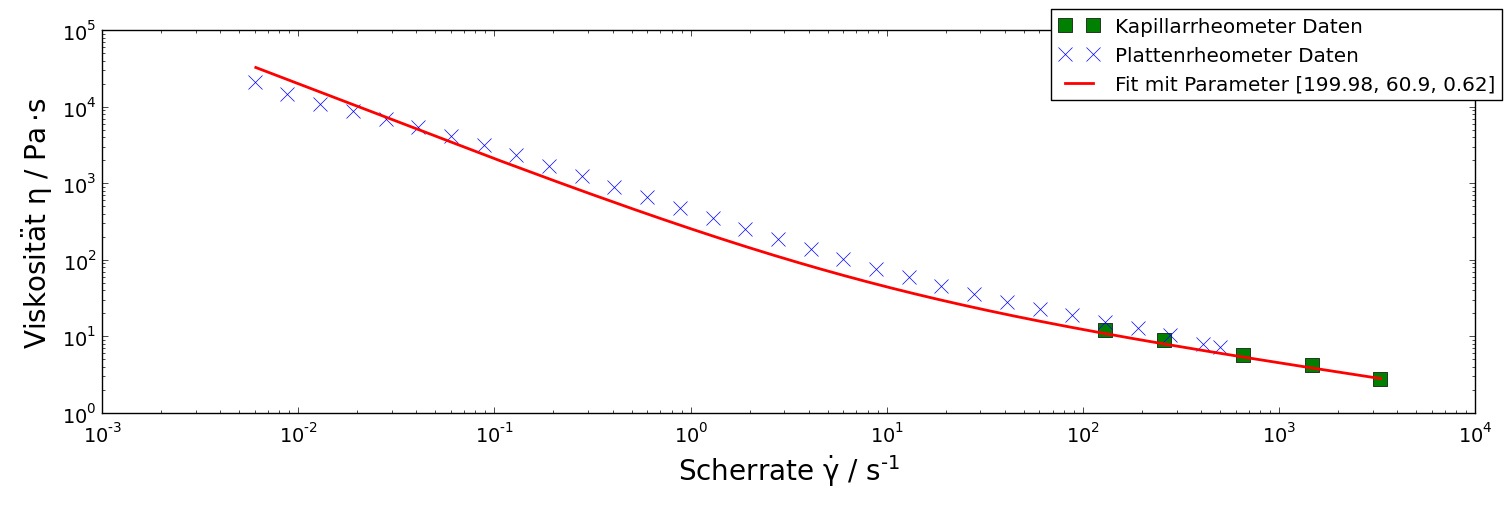
\includegraphics[width=\textwidth]{figures/shearViscoMoertel1A.png}
        \label{fig:shearViscoM1:subA}
    }\\
    \subfloat[\moertelA{} B]{
        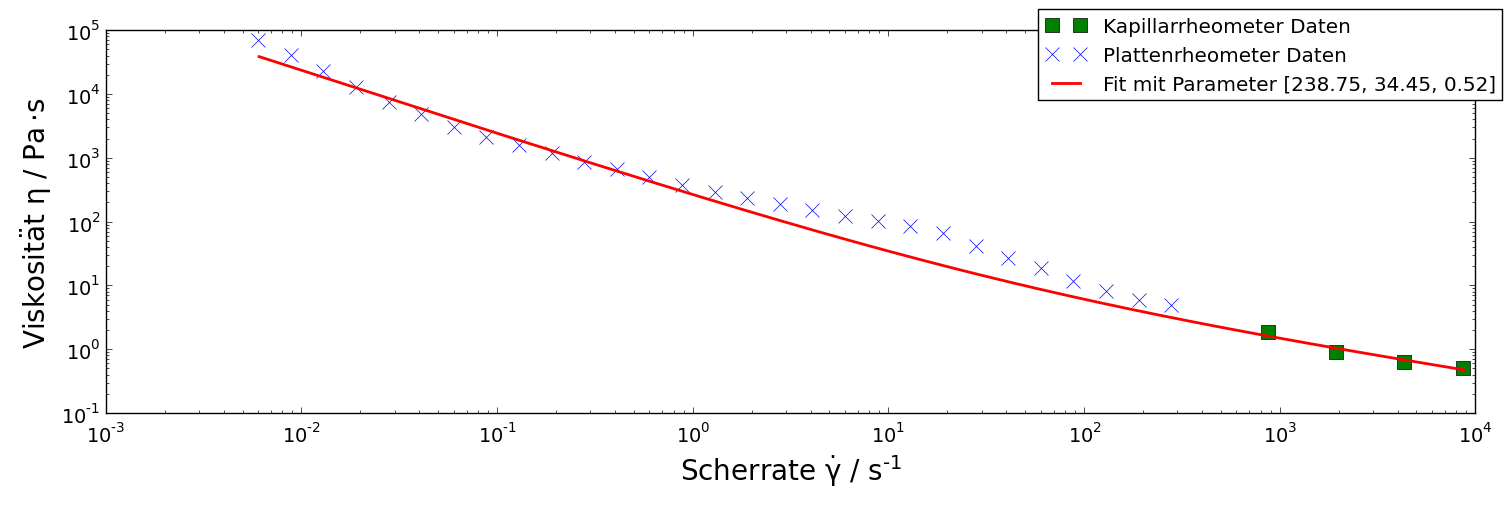
\includegraphics[width=\textwidth]{figures/shearViscoMoertel1B.png}
        \label{fig:shearViscoM1:subB}
   } \\
    \subfloat[\moertelB{} A]{
        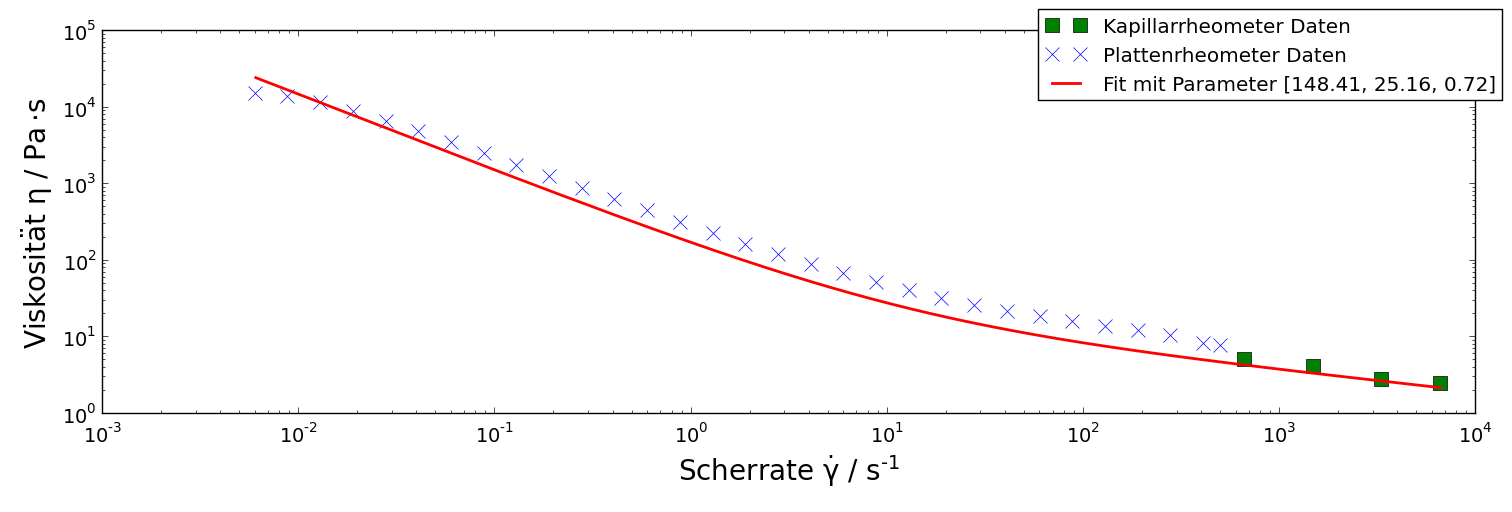
\includegraphics[width=\textwidth]{figures/shearViscoMoertel2A.png}
        \label{fig:shearViscoM2:subA}
    }\\
    \subfloat[\moertelB{} B]{
        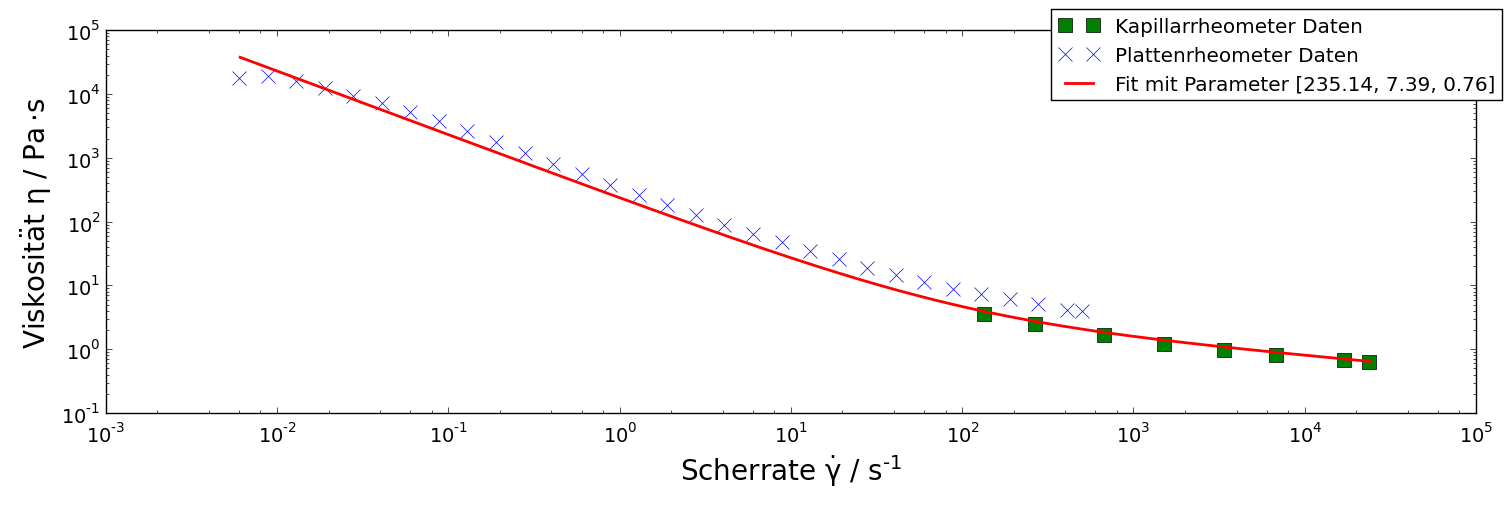
\includegraphics[width=\textwidth]{figures/shearViscoMoertel2B.png}
        \label{fig:shearViscoM2:subB}
    }
    \caption{Viskosität abhängig von der Scherrate der Mörtel. Die Kreuze und Quadrate sind Messpunkte aus den beiden Rheometern, die rote Kurve der daran angepasste Fit des Herschel-Bulkley Modells \eqref{eq:modHB}.}
    \label{fig:shearVisco}
\end{figure}
%
%\subsubsection{Relaxationszeit}

Bei den Simulationen mit dem viskoelastischen White-Metzner Materialmodell \eqref{eq:whiteMetznerModell} wird zusätzlich zu der scherratenabhängigen Viskosität auch ein Modell für die Relaxationszeit benötigt.
Das dazu verwendete Carreau-Yassuda Modell \eqref{eq:fg:carreauyasuda} besitzt die fünf Parameter $\eta_{\inf}$, $\eta_0$, $L$, $\alpha$ und $n_{\lambda}$. Da die Messung der Relaxationszeit keine Kor"-rek"-tur"-si"-mu"-la"-ti"-on benötigt, kann das Modell direkt an die Messdaten gefittet werden.
Dazu wurde ebenfalls die Python-Funktion \codeemph{leastsq} verwendet. Die resultierenden Werte sind in Tabelle \ref{fig:relaxParameter} dargestellt, in Abbildung~\ref{fig:shearLambda} sind die Messpunkte und der entsprechende Fit in einem Relaxationszeit - Scherraten Diagramm gezeigt.
\begin{table}[tbh]
    \centering
    \begin{tabular}{l c S S S S S}
        \toprule[1.5pt]
        \textbf{Mörtel} & 
        \textbf{Komponente} & 
        \multicolumn{5}{c}{\textbf{Parameter}}\\
        & &
        \multicolumn{1}{c}{$\eta_{\inf}$} & 
        \multicolumn{1}{c}{$\eta_0$} &
        \multicolumn{1}{c}{$L$} & 
        \multicolumn{1}{c}{$n_{\lambda}$} & 
        \multicolumn{1}{c}{$\alpha$} \\
        \cmidrule(lr){3-7}
        \multirow{2}{*}{\moertelA{}} & A & 0.018   & 6.81  & 3.597 & 0.015 & 2.1       \\ 
                                & B & 0.01  & 0.18  & 46.12 & 0.612 & 1.8     \\ 
        %\midrule
        %\cmidrule(lr){3-7}
        \addlinespace
        \multirow{2}{*}{\moertelB{}}  & A & 0.012 & 9.43 & 40.372  & 0.0022 & 1.643    \\ 
                                & B & 0.01   & 7.8  & 88.12  & 0.04 & 2.3         \\
        \bottomrule[1.5pt]
    \end{tabular}
    \caption{Übersicht über die verwendeten Modellparameter für das Carreau-Yasuda Modell}
    \label{fig:relaxParameter}
\end{table}
%
\begin{figure}[tb]
    \subfloat[\moertelA{} A]{
        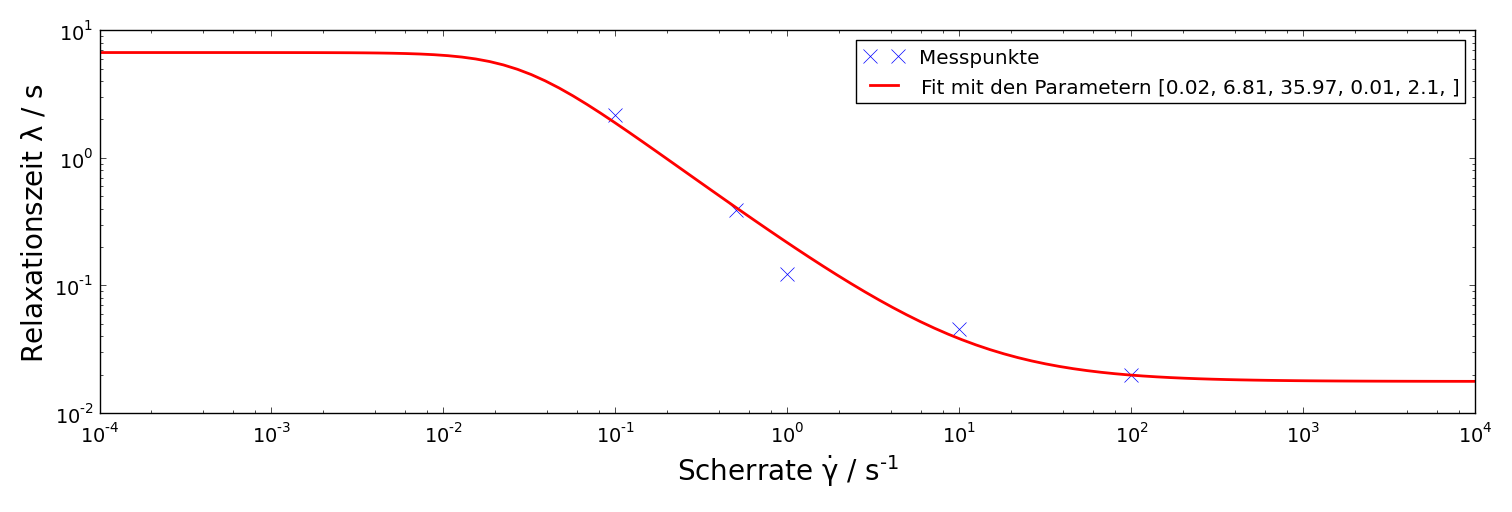
\includegraphics[width=\textwidth]{figures/shearLambdaM1A.png}
        \label{fig:shearLambdaM1:subA}
    }\\
    \subfloat[\moertelA{} B]{
        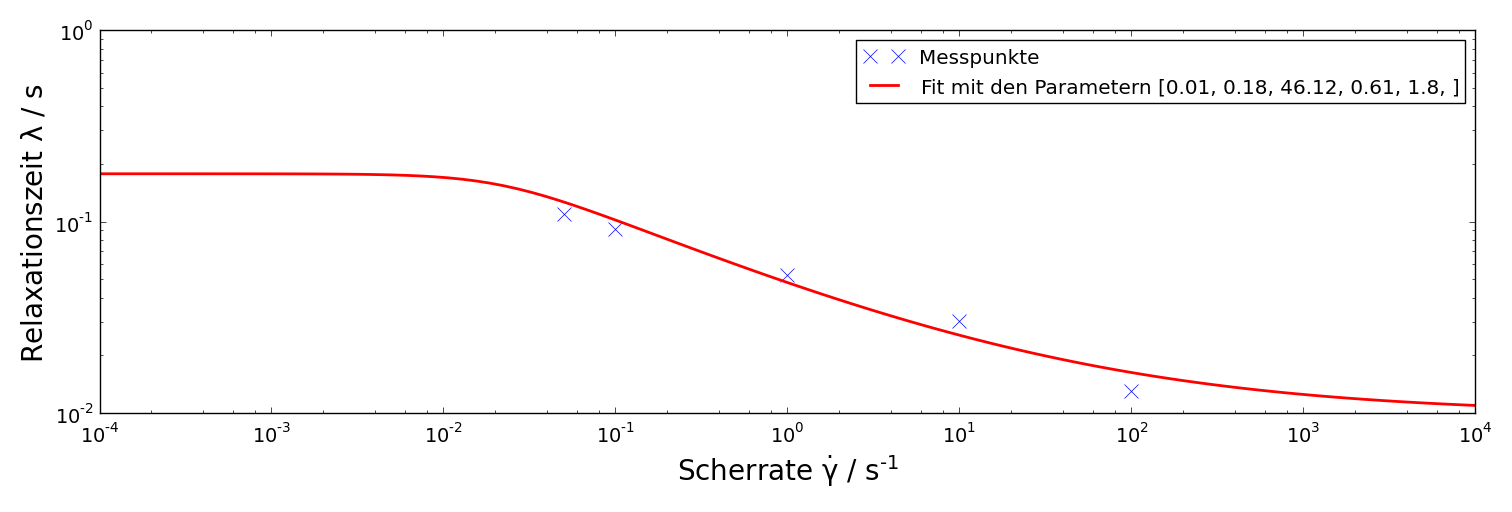
\includegraphics[width=\textwidth]{figures/shearLambdaM1B.png}
        \label{fig:shearLambdaM1:subB}
    }\\
    \subfloat[\moertelB{} A]{
        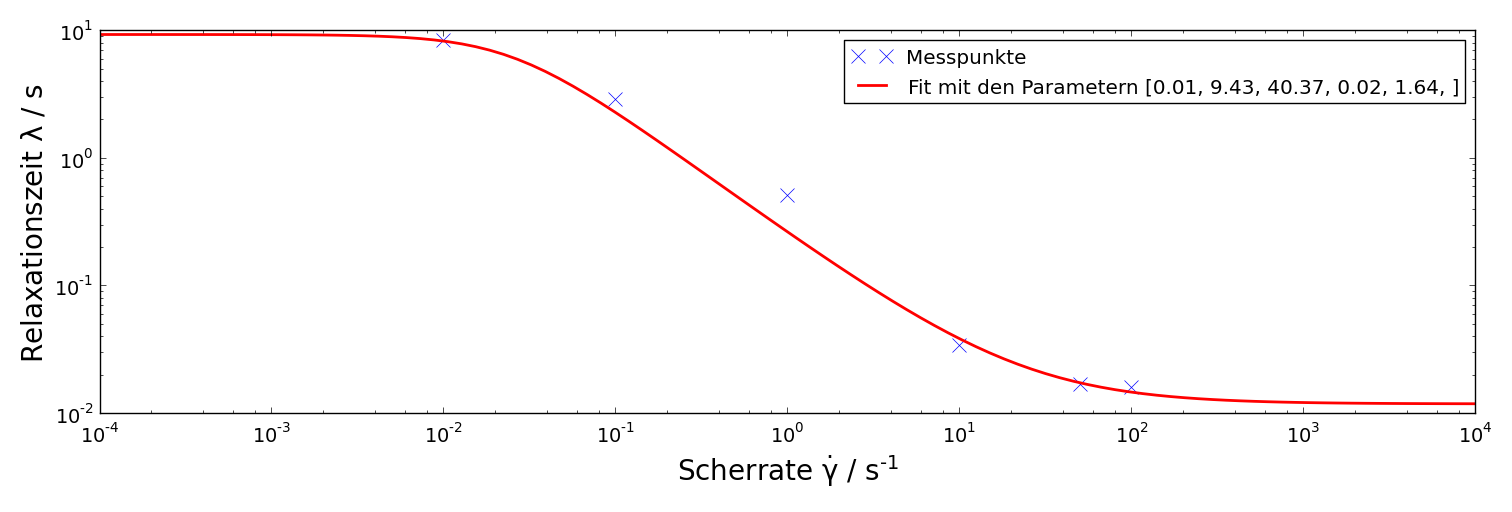
\includegraphics[width=\textwidth]{figures/shearLambdaM2A.png}
        \label{fig:shearLambdaM2:subA}
    }\\
    \subfloat[\moertelB{} B]{
        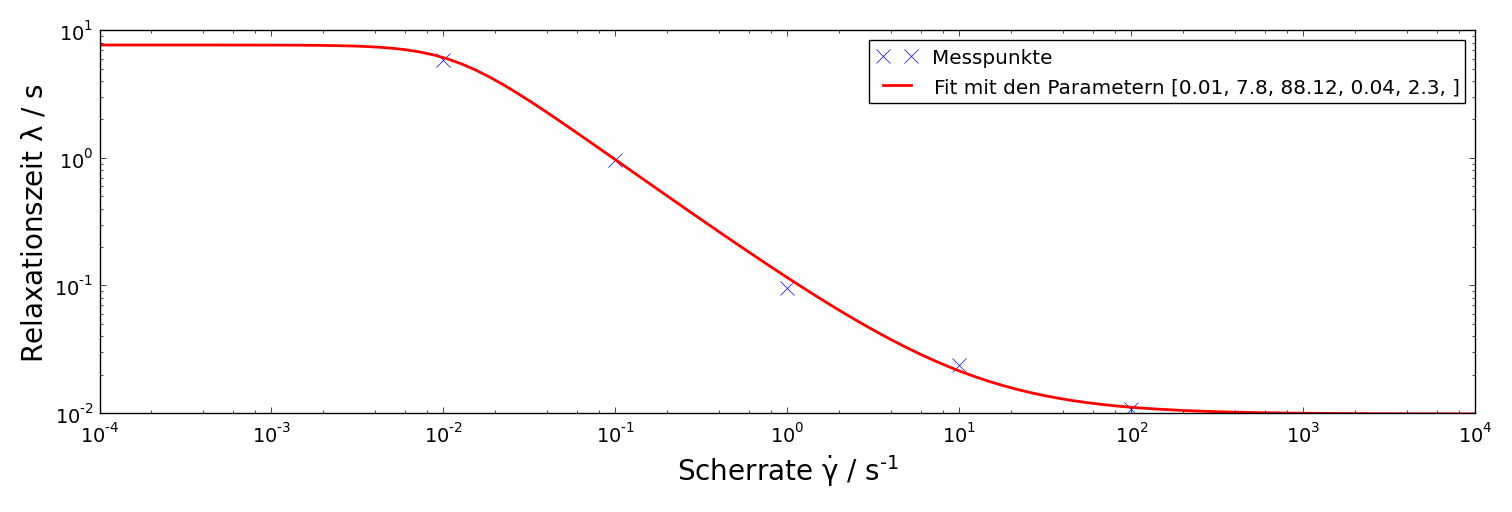
\includegraphics[width=\textwidth]{figures/shearLambdaM2B.png}
        \label{fig:shearLambdaM2:subB}
    }
    \caption{Relaxationszeit abhängig von der Scherrate der Mörtel.\\Die Kreuze sind Messpunkte aus der Rheometermessung, die rote Kurve der daran angepasste Fit des Carreau-Yasuda Modells \eqref{eq:fg:carreauyasuda}.}
    \label{fig:shearLambda}
\end{figure}
%
\FloatBarrier
\subsection{Verifikation anhand des Kapillarrheometers}
Das Kapillarrheometer musste für die Anpassung der Parameter nicht si"-mu"-liert werden. Um eine weitere Kontrollmöglichkeit über die Verlässlichkeit der Parameter zu haben, wurden deshalb Simulationen des Kapillarrheometers mit Messwerten verglichen.
Zur Vermessung des Mörtels wurden zwei Kapillarrheometer mit verschiedenen Kapillaren verwendet. 
Das eine Rheometer hat eine Kapillare der Länge von $L_\text{\tiny Kap}=\SI{32}{mm}$ und einem Durchmesser von $R_\text{\tiny Kap}=\SI{1}{mm}$, während das andere mit $L_\text{\tiny Kap}=\SI{16}{mm}$ und $R_\text{\tiny Kap}=\SI{0.5}{mm}$ eine nur halb so grosse Kapillare hat. Der Einlaufkolben ist bei beiden Rheometern gleich (Abbildung~\ref{fig:kapRheo}).
Dabei wurden sowohl Simulationen mit dem rein scherratenabhängigen Herschel-Bulkley Modell als auch mit dem viskoelastischen White-Metzner Modell durchgeführt.

\paragraph{Scherratenabhängiges Modell}
Die Simulationen mit dem scherratenabhängigen Modell wurden aufgrund der rotationssymmetrischen Geometrie ebenfalls nur für ein Segment von fünf Grad des Rheometers durchgeführt, die Randbedingungen waren dabei eine konstante Geschwindigkeit am Einlass, konstanter Druck am Auslass und Haftbedingungen an den Wänden. 
Das verwendete Netz wurde so skaliert, dass die Auflösung nahe an der Einlassdüse zur Kapillare sehr fein aufgelöst ist, während in Regionen die weit von der Düse entfernt sind, eine eher grobe Auflösung verwendet wurde. 
In Abbildung~\ref{fig:kapRheoSim} sind diese Informationen dargestellt, die Resultate sind in Tabelle \ref{fig:kapRheoResults} aufgeführt.\\
Für die beiden \moertelB{} Komponenten und die \moertelA{} A Komponente konnte eine gute Über"-einstimmung mit den Messwerten mit unter 10\% Ab\-wei\-chung erreicht werden. Beim \moertelA{} B Mörtel konnte diese Genauigkeit nicht erreicht werden. Ein möglicher Grund ist die schlechtere Qualität des Parameterfits für diesen Mörtel.
%
\begin{figure}[tb]
    \centering
    \subfloat[Randbedingungen]{
    \begin{tikzpicture} [scale=.3]
        \path[fill=lightgray] (0,0) -- (32,0) -- (32,1) -- (16,1) -- (16,7) -- (0,7) -- (0,0);
        \draw[dashed] (0,0) -- (32,0);
        \node[below] at (16,0) {Rotationssymmetrie-Achse};
        \draw[gray] (0,0) -- (0,7);
        \draw[ultra thick,<->] (3,0) -- (0,0) -- (0,3);
        \node[below] at (1.5,0) {z};
        \node[left] at (0,1.5) {r};
        \draw (32,1) -- (16,1) -- (16,7) -- (0,7);
        \node[right] at (16,4) {Wand, $\u=0$};
        \draw[->] (-8,4) -- (-1,4);
        \node[above] at (-4,4) {Einlass};
        \node[below] at (-4,4) {$\u$ konstant};
        \draw[gray] (32,0) -- (32,1);
        \draw[->] (32.5,.5) -- (36,.5);
        \node[above] at (34.5,0.5) {Auslass};
        \node[below] at (34.5,0.5) {$p$ konstant};
    \end{tikzpicture}
    \label{fig:kapRheoSim:subA}
    }\\
    \subfloat[Netz]{
    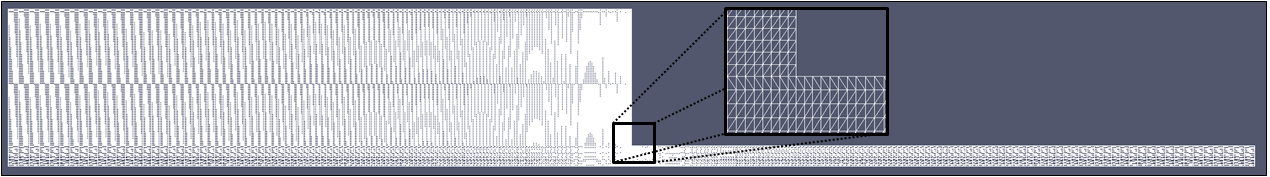
\includegraphics[width=\textwidth]{figures/kapRheoSimNetzZoom.PNG}
    \label{fig:kapRheoSim:subB}
    }\\
    \subfloat[Resultat]{
    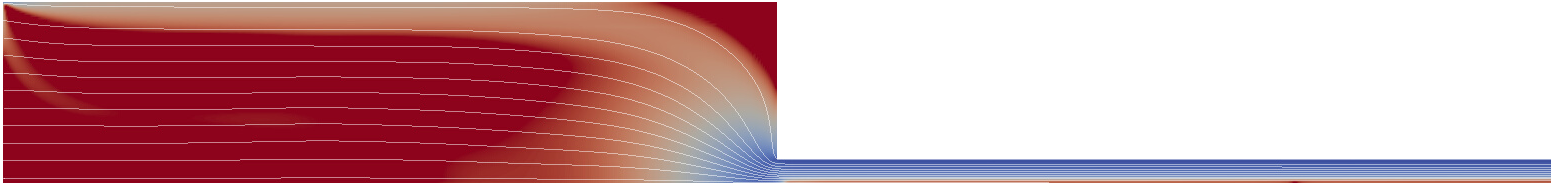
\includegraphics[width=\textwidth]{figures/kapRheoSimResult.PNG}
    \label{fig:kapRheoSim:subC}
    }
    \caption{Der mit dem Herschel-Bulkley Modell simulierte Teil des Kapillarrheometers. In \subref{fig:kapRheoSim:subA} sind die Randbedingungen gegeben. In \subref{fig:kapRheoSim:subB} ist das Netz dargestellt. Dabei handelt es sich um ein Hexaeder-Netz, trotz der Darstellung mit Dreiecken. Diese stammt von Paraview. In \subref{fig:kapRheoSim:subC} ist das Resultat der Simulation zu sehen. Dargestellt ist ein Farbplot der Viskosität (blau: flüssig, rot: zäh); die Stromlinien sind in Weiss eingetragen.}
    \label{fig:kapRheoSim}
\end{figure}
%
\begin{table}[bt]
    \centering
    \begin{tabular}{l S S S S}
        \toprule[1.5pt]
        \multicolumn{2}{c}{\textbf{Messaufbau}} & 
        \multicolumn{2}{c}{\textbf{Druckverlust}} & 
        \multicolumn{1}{l}{\textbf{Fehler}} \\

        \multicolumn{1}{l}{\textbf{Mörteltyp}}& 
        \multicolumn{1}{c}{$\u$} & 
        \multicolumn{1}{l}{\textbf{Messung}} & 
        \multicolumn{1}{l}{\textbf{Simulation}} &
        \\
        & 
        \multicolumn{1}{r}{\si{mm/s}} & 
        \multicolumn{1}{r}{\si{Bar}} & 
        \multicolumn{1}{r}{\si{Bar}} &
        \multicolumn{1}{r}{\si{\%}}
        \\
        %\cmidrule(r){1-1}
        \cmidrule(lr){1-2}
        \cmidrule(lr){3-4}
        \cmidrule(lr){5-5}
        \multirow{5}{*}{\moertelA{} A} & 0.53 & 0.98 & 1.06 &  6.98\\
                                  & 1.07 & 1.46 & 1.53 &  4.74\\
                                  & 2.67 & 2.42 & 2.54 &  4.53\\
                                  & 6.02 & 4.22 & 4.09 &  3.13\\
                                  & 13.4 & 6.27 & 6.59 &  4.76\\
        \cmidrule(lr){1-2}
        \cmidrule(lr){3-4}
        \cmidrule(lr){5-5}
        \multirow{5}{*}{\moertelA{} B} & 0.13 & 0.55 & 0.64 &  13.95\\
                                  & 0.33 & 1.09 & 1.36 &  19.68\\
                                  & 0.75 & 1.33 & 1.36 &   2.04\\
                                  & 1.67 & 2.13 & 1.90 &  11.82\\
                                  & 3.34 & 3.12 & 2.65 &  17.58\\
        \cmidrule(lr){1-2}
        \cmidrule(lr){3-4}
        \cmidrule(lr){5-5}
        \multirow{5}{*}{\moertelB{} A}  & 0.13 &  1.15 &  1.18  & 2.16\\
                                  & 0.33 &  2.35 &  2.37  & 0.65\\
                                  & 0.75 &  4.22 &  4.18  & 1.01\\
                                  & 1.67 &  6.56 &  7.21  & 8.95\\
                                  & 3.34 & 11.51 & 11.93  & 3.49\\
        \cmidrule(lr){1-2}
        \cmidrule(lr){3-4}
        \cmidrule(lr){5-5}
        \multirow{5}{*}{\moertelB{} B}  & 0.13 & 1.04 & 0.95 &  9.78\\
                                  & 0.33 & 1.53 & 1.56 &  1.92\\
                                  & 0.75 & 2.62 & 2.56 &  6.54\\
                                  & 1.67 & 4.22 & 4.03 &  4.77\\
                                  & 3.34 & 6.19 & 6.42 &  3.66\\
        \bottomrule[1.5pt]
    \end{tabular}
    \caption{Die Messungen und Resultate der Kapillarrheometer-Simulation. Dabei wurde für den \moertelA{} A die \SI{2}{mm} Kapillare, für die anderen Mörtel die \SI{1}{mm} Kapillare verwendet.}
    \label{fig:kapRheoResults}
\end{table}

\paragraph{Viskoelastisches Modell}
Für die viskoelastischen Simulationen konnte nicht nur ein Segment des Kapillarrheometers verwendet werden, da die 'wedge'-Randbedingung \footnote{Randbedingung, die von \openfoam{} für Front und Rückseite einer rotationssymmetrischen Geometrie verwendet wird.} von \openfoam{} die Resultate verfälschte. Daher wurde ein Netz des ganzen Rheometers erstellt und die Simulationen damit durchgeführt.

Der für viskoelastische Fluide typische Wirbel bei einer plötzlichen Verengung der Fliessgeometrie \cite{Evans198611} konnte so erfolgreich nachgebildet werden. Abbildung~\ref{kapRheoVisco} zeigt das Auftreten dieses Wirbels in einer Kapillarrheometer Simulation.
%
\begin{figure}
    \centering
    \subfloat[Druckverlauf mit Stromlinien]{
    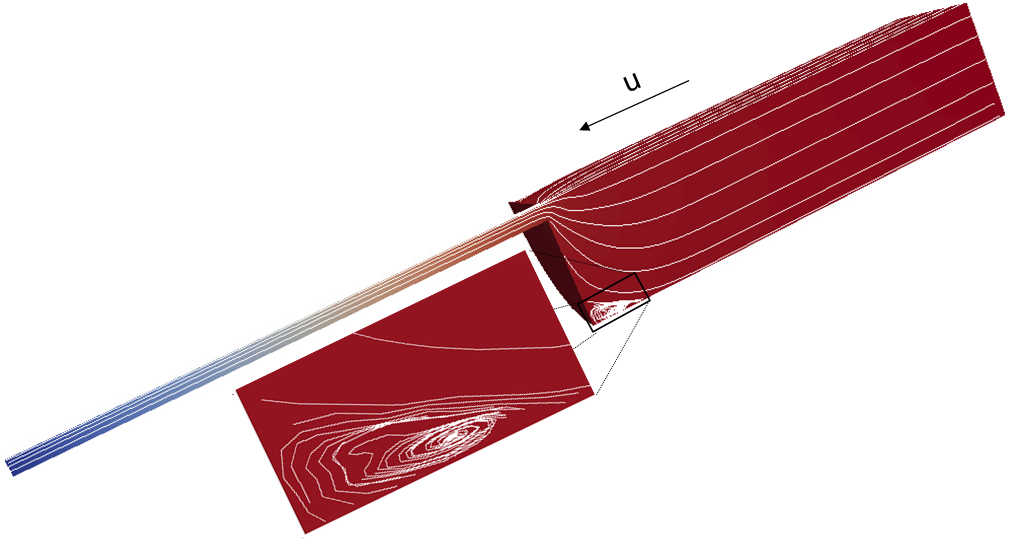
\includegraphics[width=\textwidth]{figures/kapRheoSimP.PNG}
    \label{fig:kapRheoVisco:subA}
    }\\
    \subfloat[Schubspannung]{
    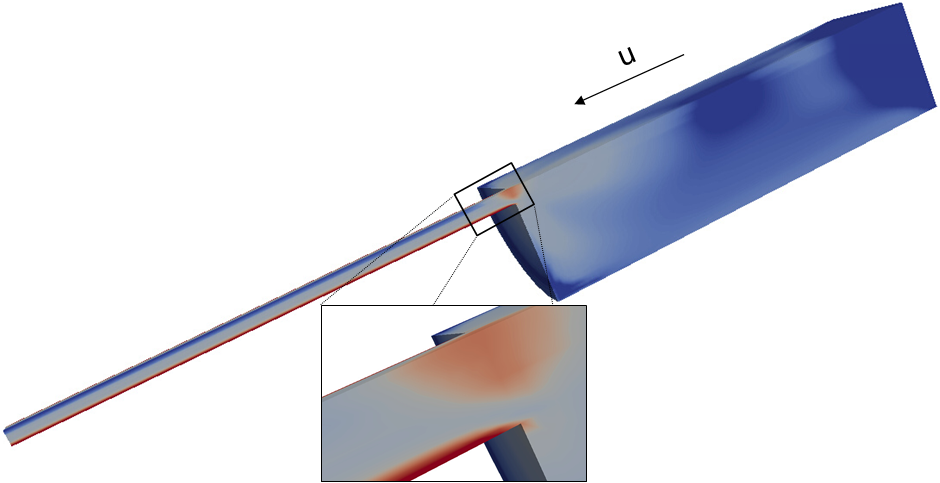
\includegraphics[width=\textwidth]{figures/kapRheoSimTau.PNG}
    \label{fig:kapRheoVisco:subB}
    }
    \caption{Viskoelastische Simulation des Kapillarrheometers. Die Vergrösserung in \subref{fig:kapRheoVisco:subA} zeigt den sich bildenden Wirbel in der laminaren Strömung, der auf die Visko\-elastizität zurückzuführen ist. Das Rheometer ist nach dem Druckverlauf eingefärbt (blau: tief, rot: hoch). Abbildung~\subref{fig:kapRheoVisco:subB} ist nach der berechneten Schubspannung eingefärbt. In der Kapillare nimmt sie in radialer Richtun zu, beim Einlass bildet sich ein Gebiet erhöhter Schubspannung durch die Verengung des Querschnittes.}
    \label{kapRheoVisco}
\end{figure}
%

Die Simulation des Kapillarrheometers mit dem scherratenabhängigen \linebreak Herschel-Bulkley Modell zeigt eine gute Übereinstimmung mit den Messdaten.
Das viskoelastische Modell konnte ebenfalls erfolgreich für eine Simulation des Kapillarrheometers verwendet werden.
Um den Einfluss der Viskoelastizität auf den Druckverlust zu testen, wurde für alle Mörteltypen eine Rechnung jeweils mit und ohne viskoelastischem Modell gerechnet. Die Resultate sind in Tabelle~\ref{fig:einflussVisko} aufgeführt.
%
\begin{table}[bt]
\noindent\makebox[\textwidth]{%
    \centering
    \begin{tabular}{l S S S S}
        \toprule[1.5pt]
        \textbf{Rheologisches Verhalten}&\multicolumn{4}{c}{\textbf{$\Delta p$} in Bar}
        \\
        &
        \multicolumn{1}{l}{\textbf{\moertelA{} A}}& 
        \multicolumn{1}{l}{\textbf{\moertelA{} B}}& 
        \multicolumn{1}{l}{\textbf{\moertelB{} A}}& 
        \multicolumn{1}{l}{\textbf{\moertelB{} B}}
        \\
        \cmidrule(lr){2-5}
        Scherratenabhängig  & 0.5777 & 0.3699 & 0.3757 & 0.2931 \\
        Viskoelastisch & 0.5850 & 0.4098 & 0.3805 & 0.2869 \\
        \bottomrule[1.5pt]
    \end{tabular}}
    \caption{Der Einfluss der Viskoelastizität auf den Druckverlust. In der oberen Zeile die Simulationen mit den rein scherratenabhängigen Modellen, unten mit berücksichtigter Viskoelastizität. Für die Simulation wurde das Kapillarrheometer mit \SI{2}{mm} Kapillare und einer Einlassgeschwindigkeit von \SI{0.13}{mm.s^{-1}} verwendet.}
    \label{fig:einflussVisko}
\end{table}

Aufgrund der schwachen viskoelastischen Eigenschaften der Mörtel sind die Einflüsse auf den Druckverlust nur minimal. Da die benötigte Rechenzeit bei der Verwendung des viskoelastischen Modells sehr stark ansteigt, wurde darauf verzichtet die weiteren Rechnungen damit durchzuführen.
